\begin{frame}
    \frametitle{Visualizzare ed Elaborare documenti XML}
    \addtocounter{nframe}{1}
    
    %\begin{center}
    %    
\includegraphics[width=.2\textwidth]{../imgs/tei-r.pdf}
    %\end{center}
    %\textit{In parte già disponibili nei moduli TEI di base}

     \begin{block}{Perché visualizzare il testo}
    %     \emph{Per la critica testuale indispensabili i moduli}
         \begin{itemize}
            \item  Controllare la codifica e correggere i refusi
             \item Assicurarsi che tutto sia stato trascritto correttamente
             \item Mostrare il testo a persone che non conoscono XML-TEI
             \item Disporre di una versione del lavoro fuibile
        \end{itemize}
     \end{block}
    
\end{frame}

\begin{frame}
    \frametitle{Visualizzare ed Elaborare documenti XML}
    \addtocounter{nframe}{1}
    
    \begin{center}
        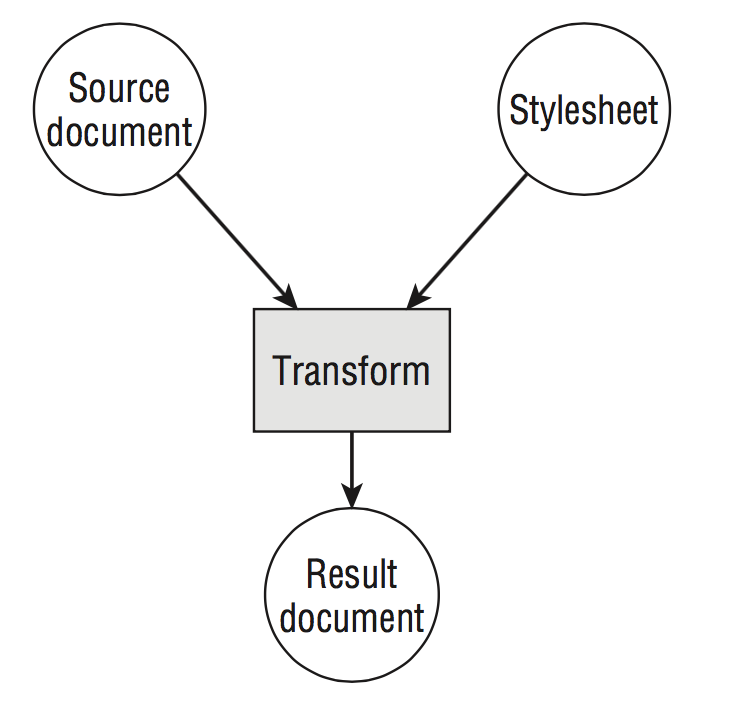
\includegraphics[width=.9\textwidth]{imgs/SchemaXSLTprocessing.png}
    \end{center}
    %\textit{In parte già disponibili nei moduli TEI di base}

\end{frame}

% Controllo e gestione degli spazi bianchi p 54 slide di Chiara